\section{Compute Hardware}

\begin{frame}{Parallel Computations}
\begin{center}
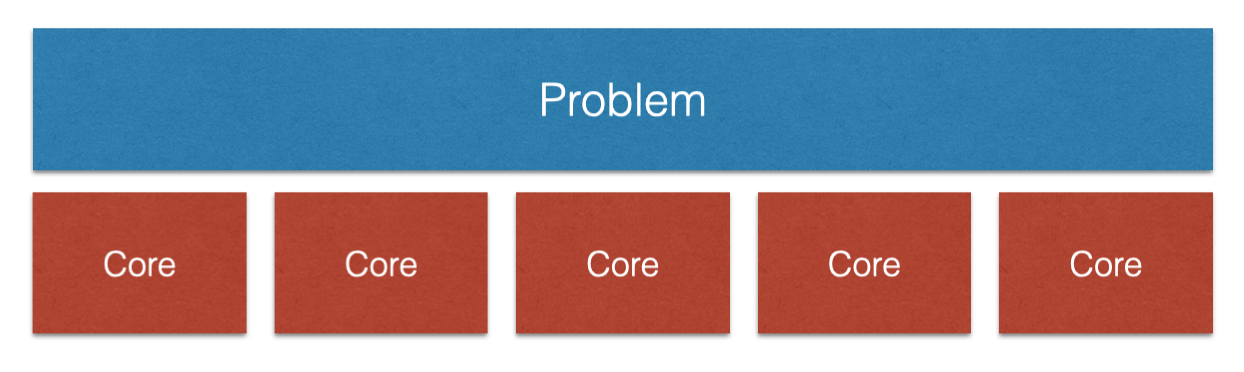
\includegraphics[width=0.65\linewidth]{figures/problem_over_cores.png}
\end{center}
\begin{itemize}
\item Using multiple processing units (cores, etc.) simultaneously to perform a computation
\item Use multiple computers to store data for large problems
\item Essentially all modern CPUs have multiple cores
\end{itemize}
\end{frame}

\begin{frame}{Parallel Hardware}
\begin{itemize}
\item Levels of parallelism
\item Vectorization
\item Multicore
\item Multi-CPU
\item Multi-Node
\item Threads versus processes
\end{itemize}
\end{frame}

\begin{frame}{Intel Xeon Phi Nodes}
\begin{columns}
\begin{column}{0.5\textwidth}
\begin{itemize}
\item Intel Xeon Phi 7230 (also known as ``Knights Landing'' or ``KNL'') processors
\item 64 1.30 GHz cores based on the Atom ``Silvermont'' architecture
\item Cache: 32 MB L2
\item Cache: 16 GB of high bandwidth (400 GB/s) stacked memory
\item Memory: DDR4 2400 MHz, 115.2 GB/s
\item Vector Extensions: AVX-512 (512 bit width)
\item Hardware-based support for up to four concurrent threads
\end{itemize}
\end{column}
\begin{column}{0.5\textwidth}
\begin{center}
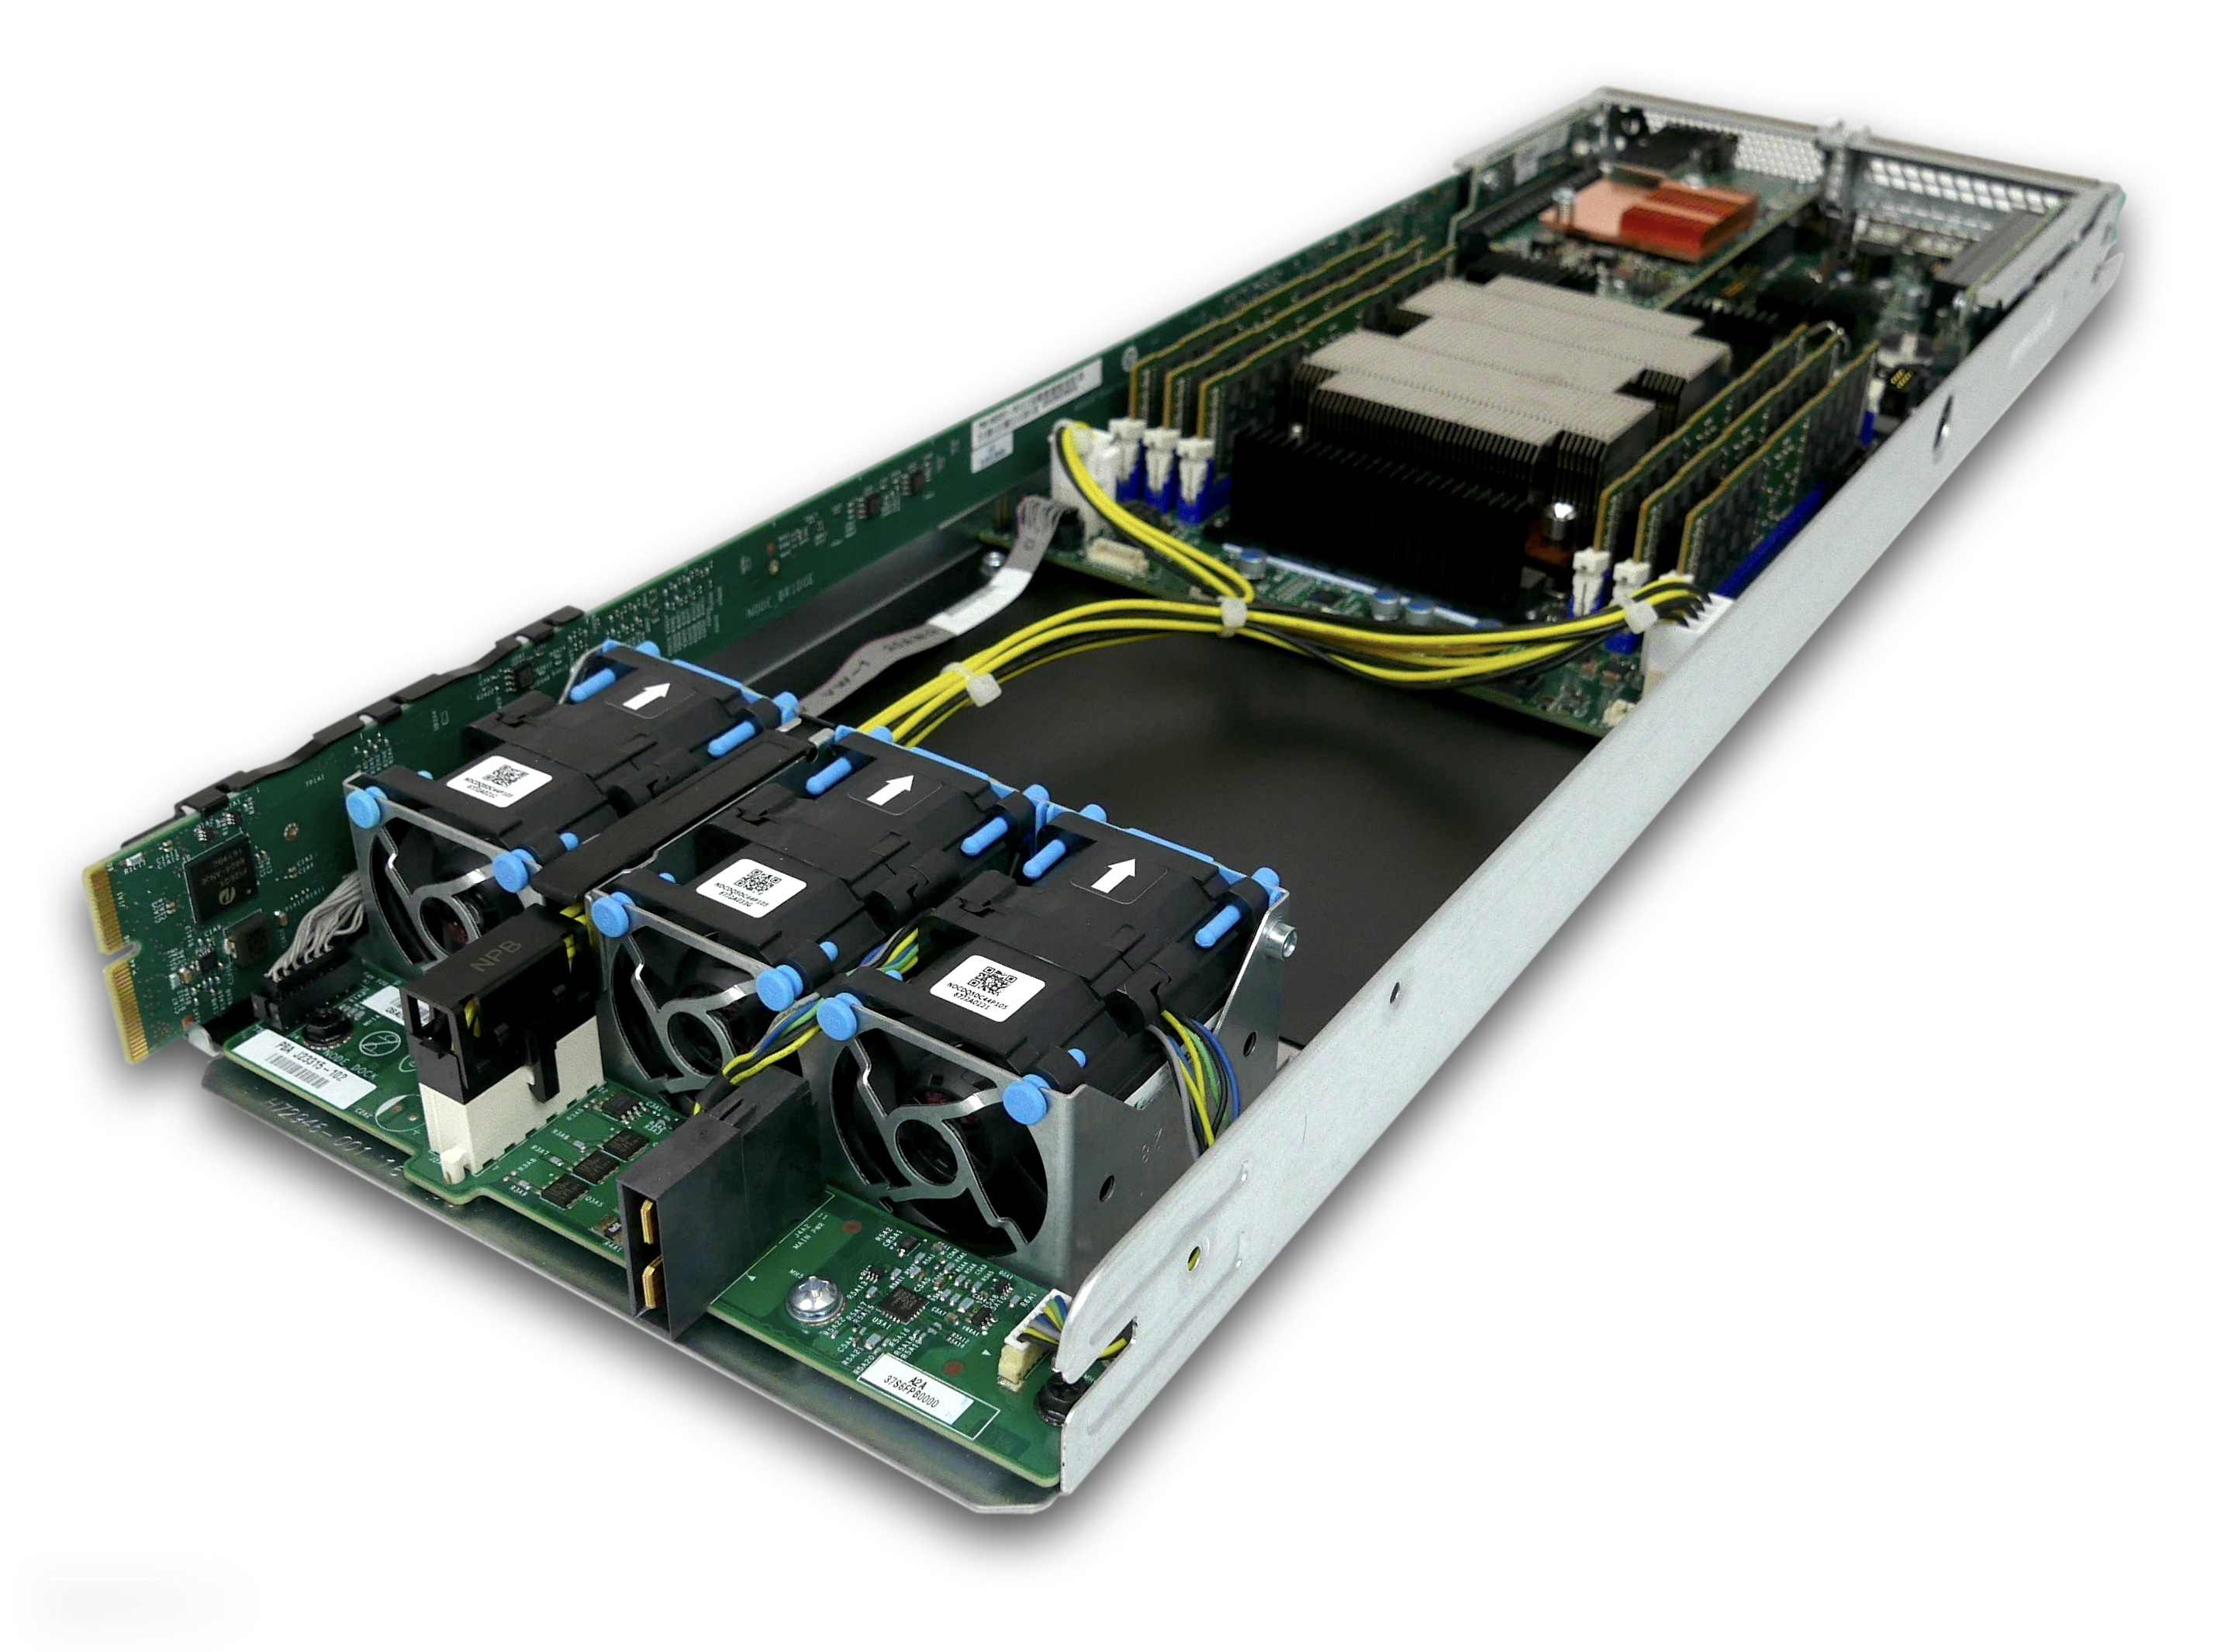
\includegraphics[width=\textwidth]{figures/mic_sled.jpg}
\end{center}
\end{column}
\end{columns}
\end{frame}

\begin{frame}{Intel Xeon Phi Nodes}
\begin{center}
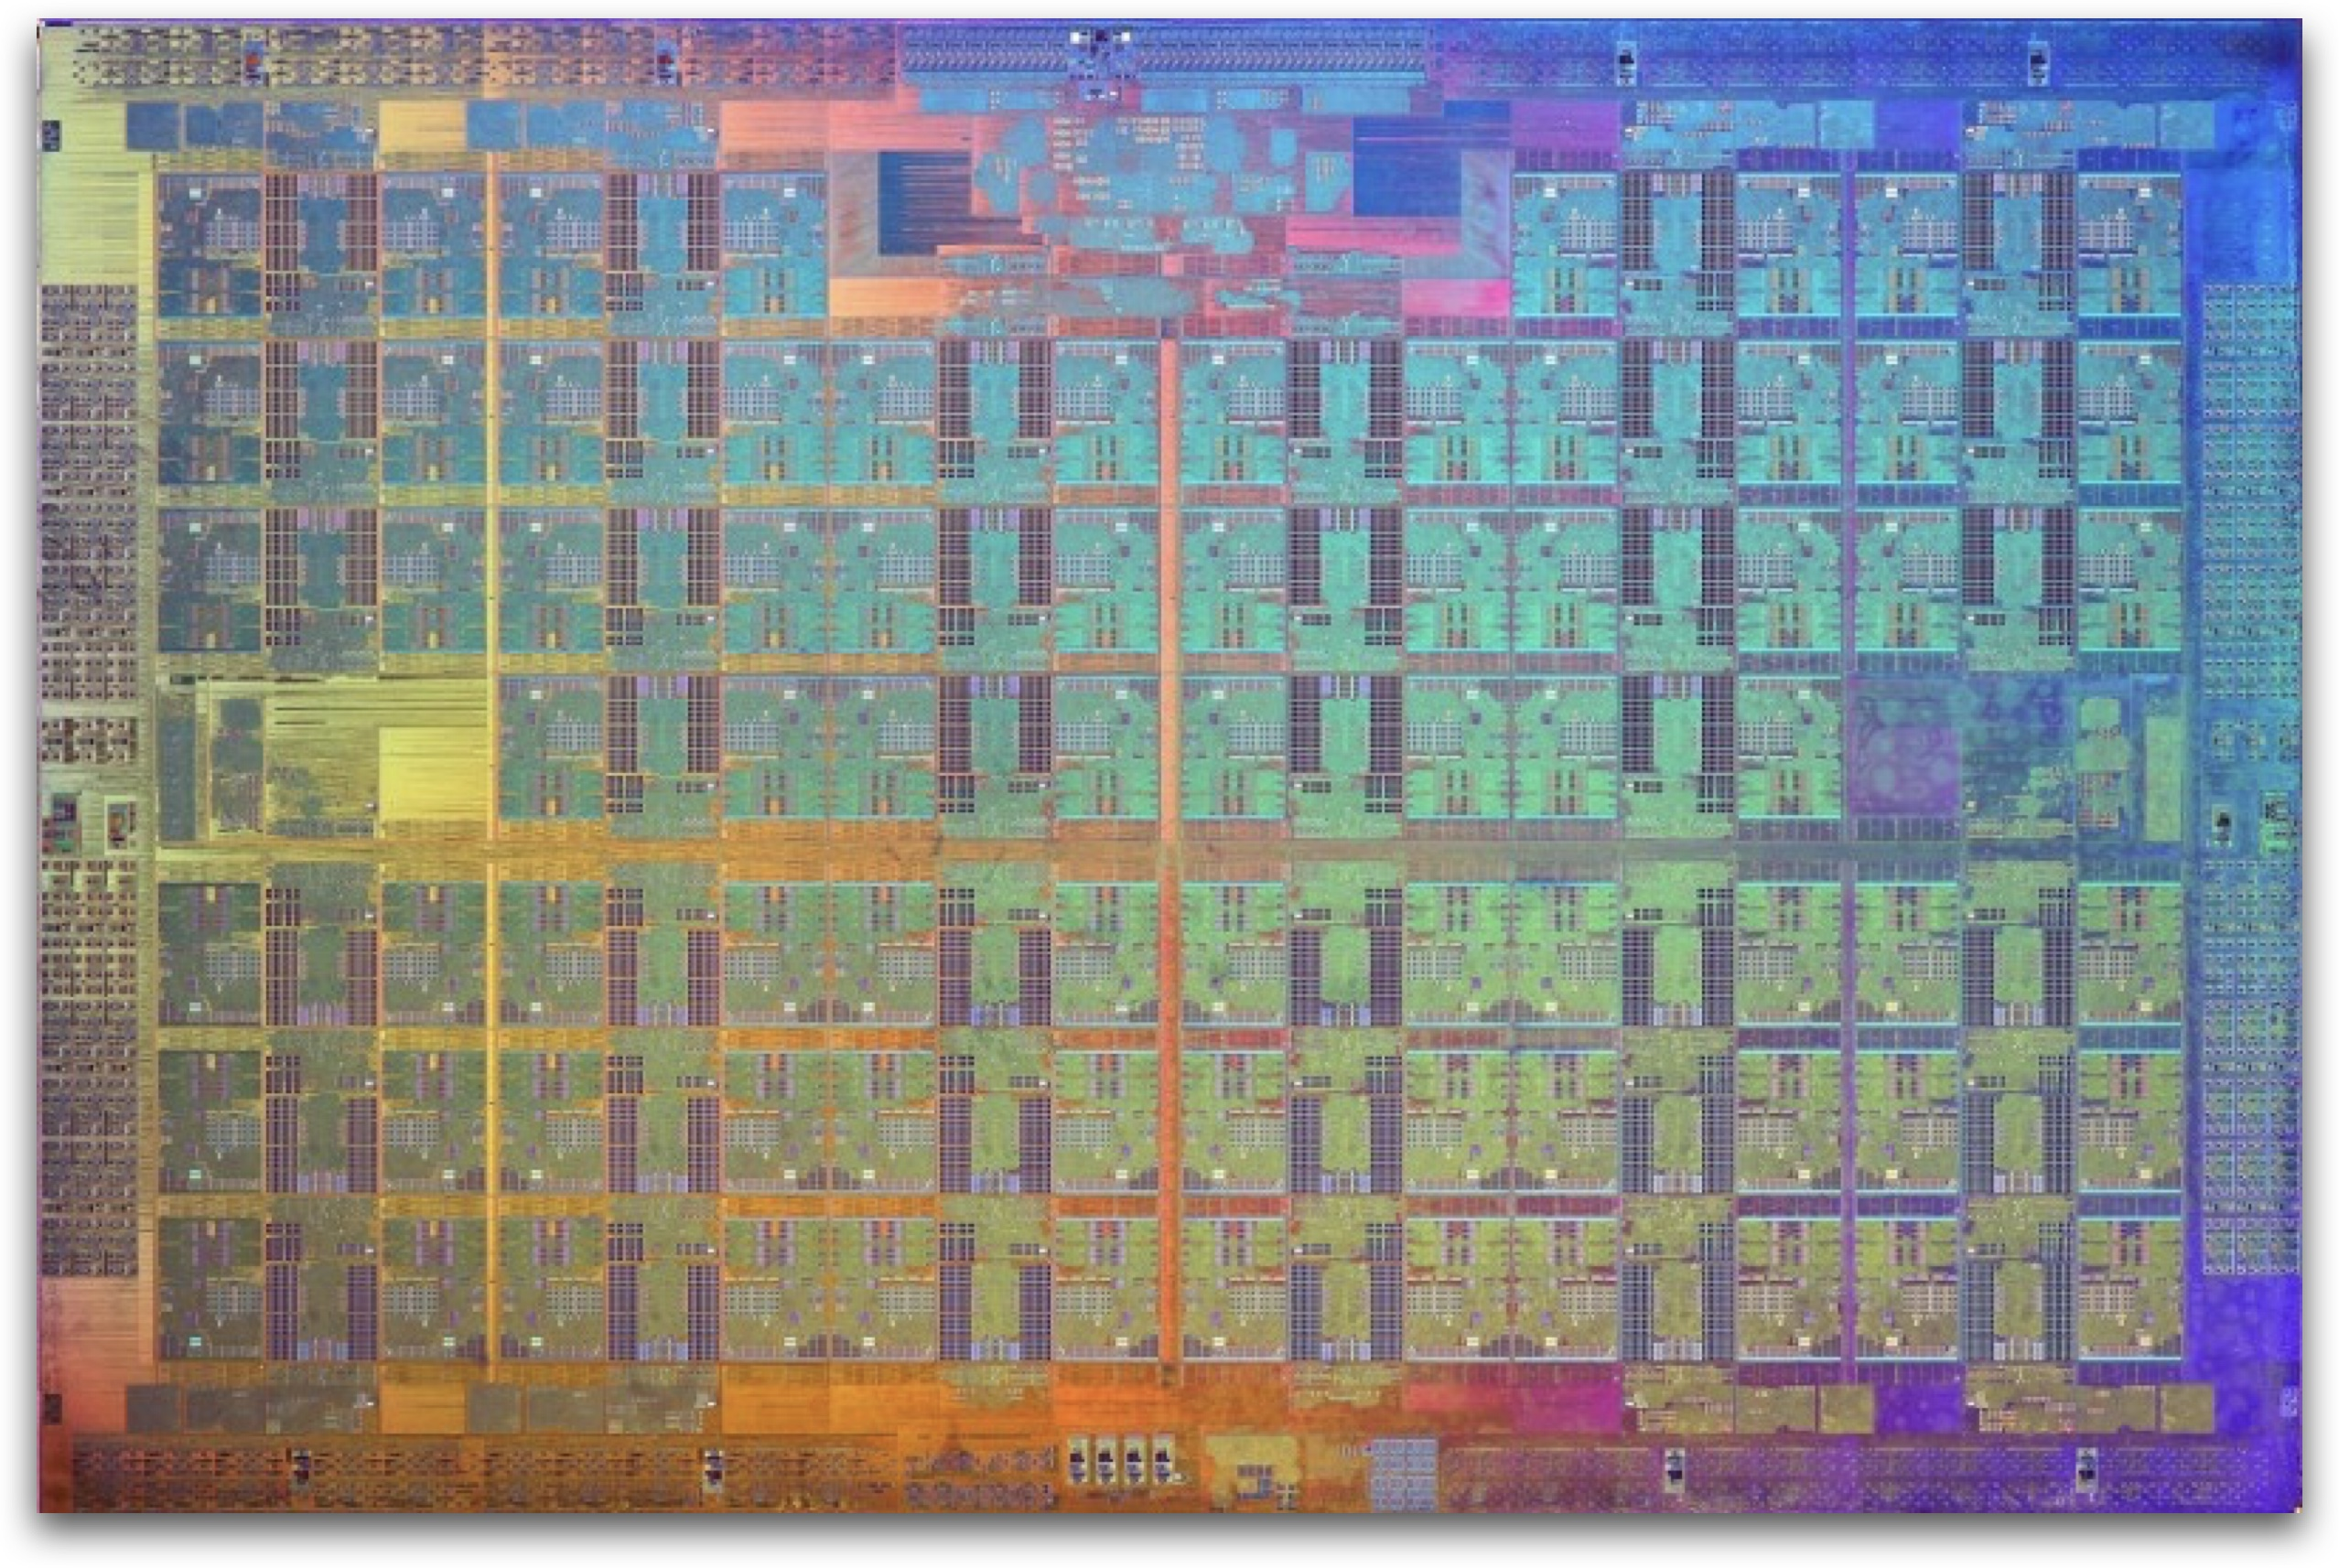
\includegraphics[height=0.75\textheight]{figures/mic_die_shot.jpg}
\end{center}
\end{frame}

\begin{frame}{Intel Xeon “Broadwell” Nodes}
\begin{itemize}
\item Dual Intel Xeon E5-2695v4 2.1 GHz 18-core ``Broadwell'' processors
\item Cache: 45 MB L3
\item Memory: DDR4 2400 MHz, 76.8 GB/s
\item Vector Extensions: AVX2 (256 bit width)
\end{itemize}
\end{frame}

\begin{frame}{Intel Xeon “Skylake” Nodes}
\begin{itemize}
\item Dual Intel Xeon Gold 6154 3.0 GHz 18-core ``Skylake'' processors
\item Cache: 24.75 MB L3
\item Memory: DDR4 2666 MHz, 119.21 GB/s
\item Vector Extensions: AVX-512 (512 bit width)
\end{itemize}
\end{frame}

\begin{frame}{NVIDIA SuperPOD DGX Nodes}
\begin{columns}
\begin{column}{0.5\textwidth}
\begin{itemize}
\item Dual AMD Epyc 7742 2.25 GHz 64-core ``Rome'' processors
\item Cache: 256 MB L3
\item Memory: DDR4 3200 MHz, 204.8 GB/s
\item Vector Extensions: AVX2 (256 bit width)
\end{itemize}
\end{column}
\begin{column}{0.5\textwidth}
\begin{center}
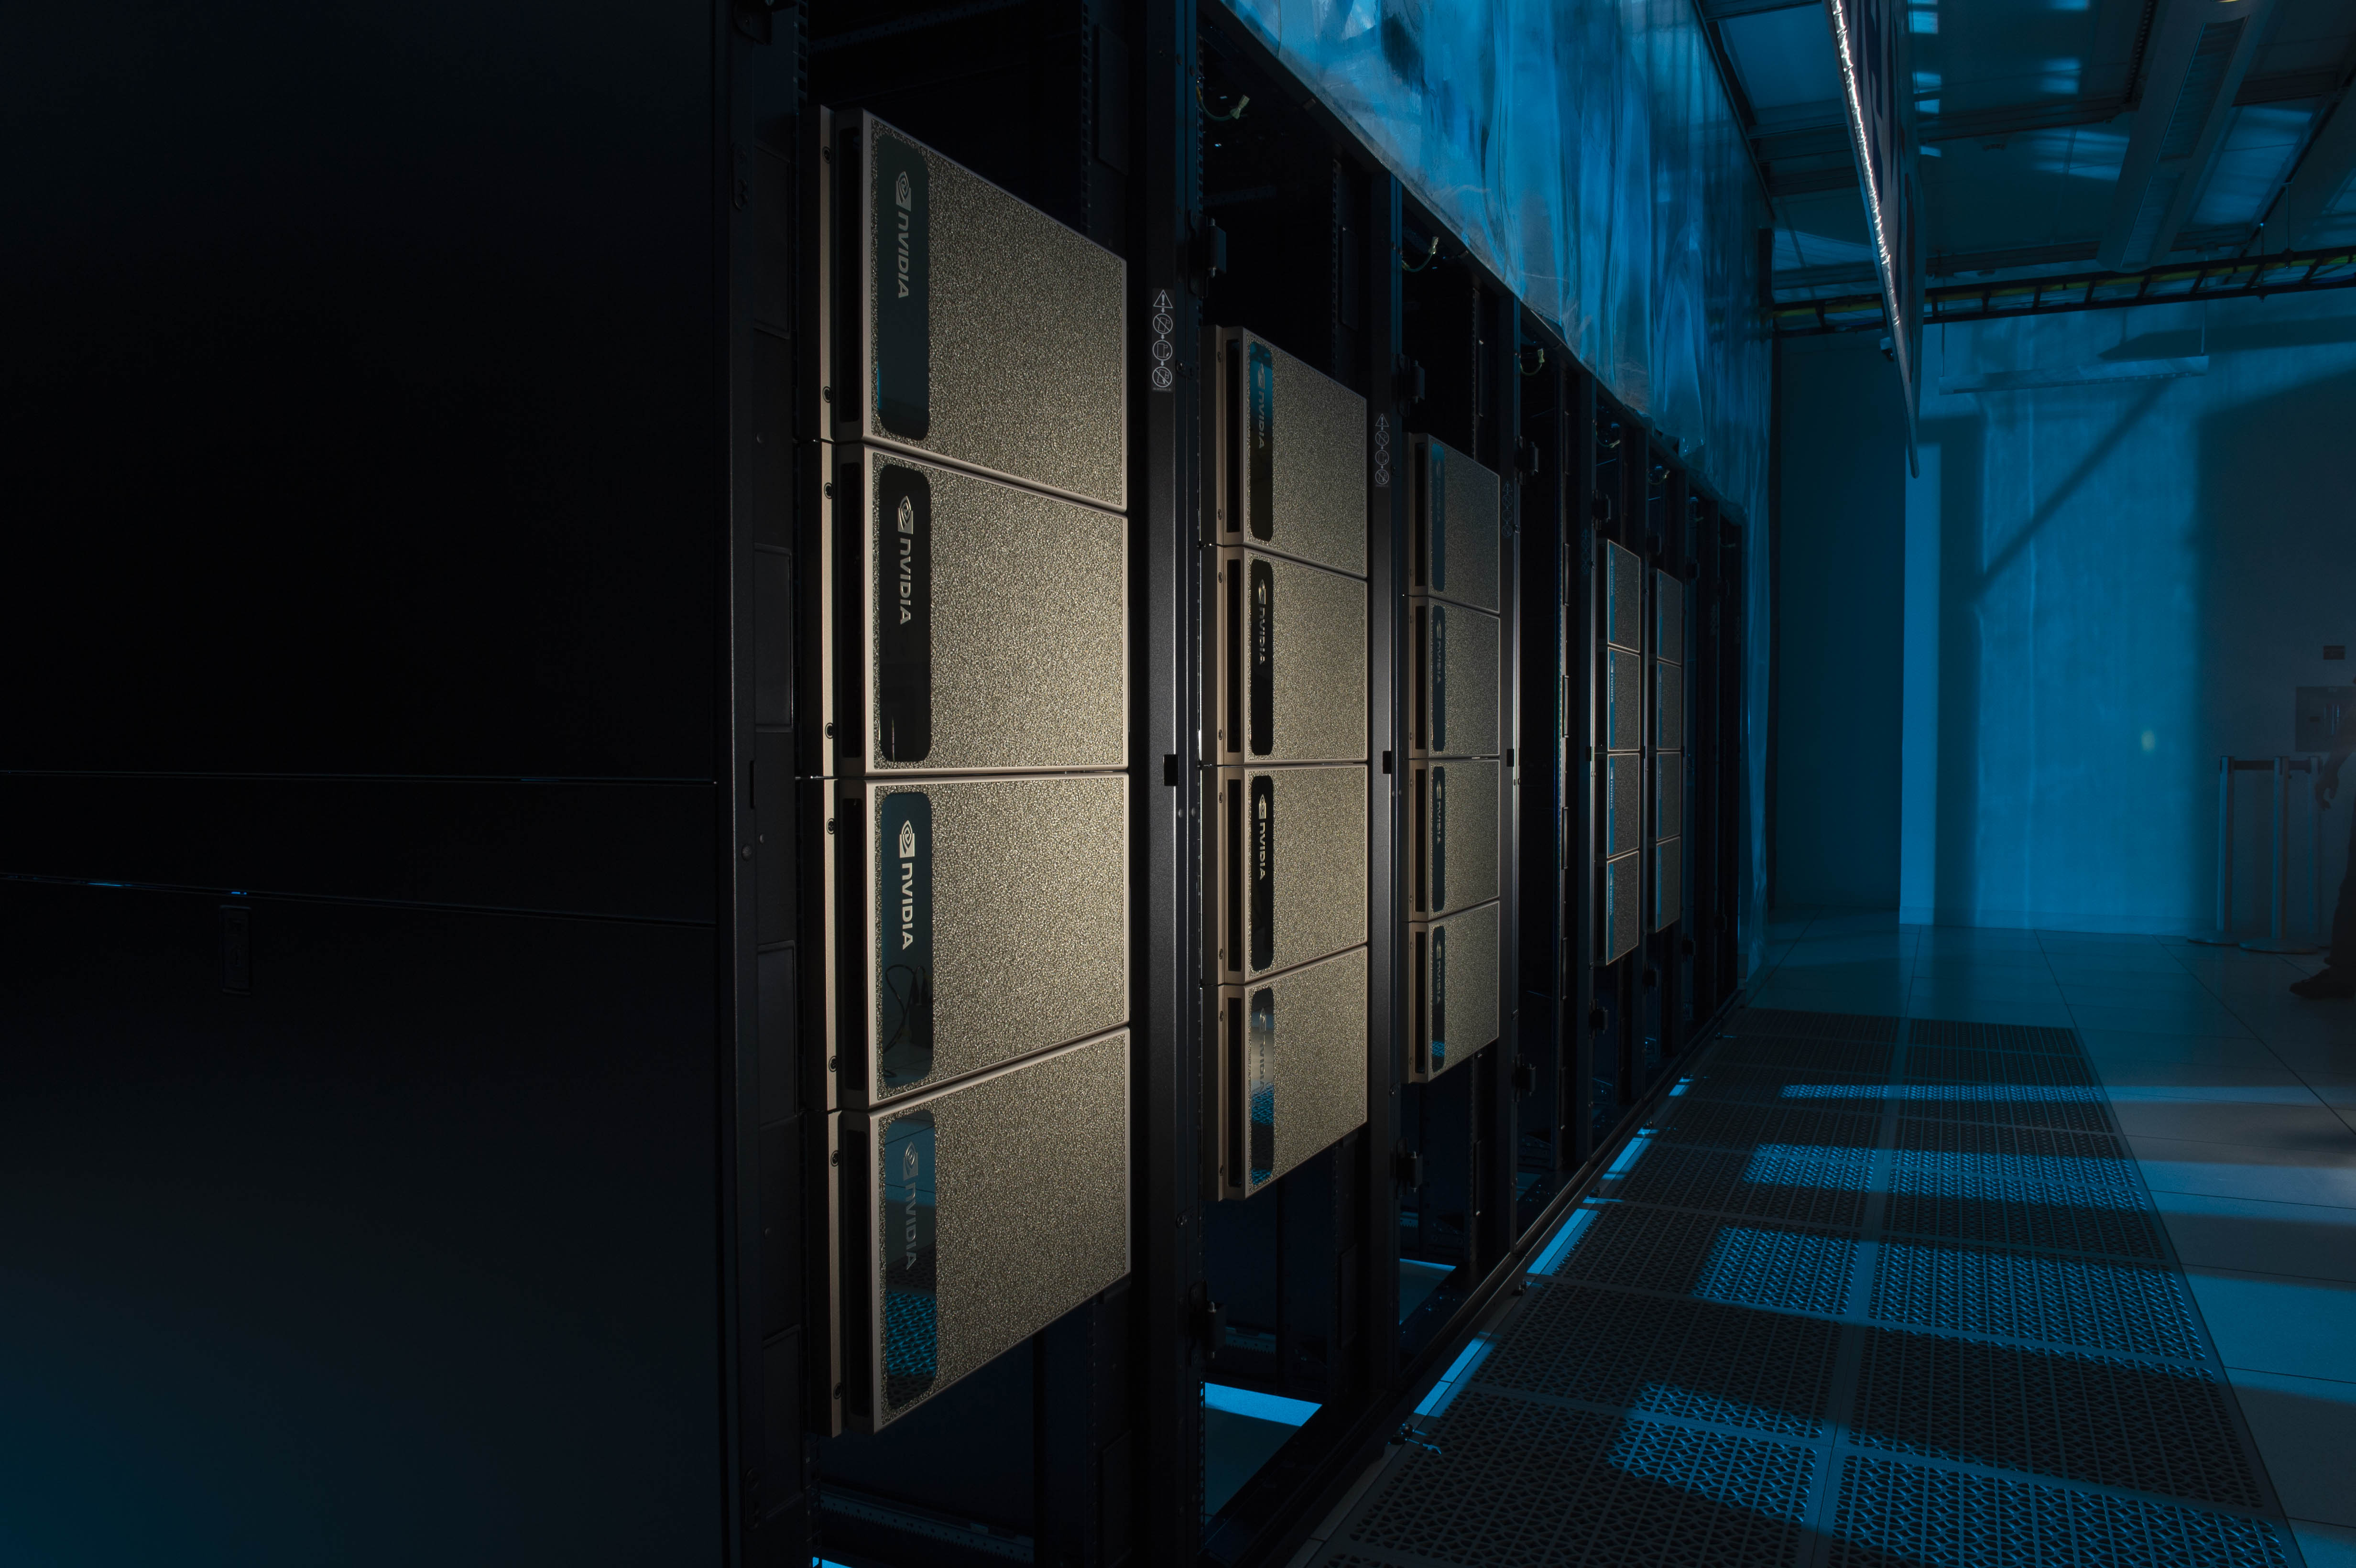
\includegraphics[width=\textwidth]{figures/superpod.jpg}
\end{center}
\end{column}
\end{columns}
\end{frame}

